% $Header: /home/vedranm/bitbucket/beamer/solutions/generic-talks/generic-ornate-15min-45min.en.tex,v 90e850259b8b 2007/01/28 20:48:30 tantau $

\documentclass{beamer}
%\documentclass[handout]{beamer}
%\usepackage{pgfpages}
%\usepackage{handoutWithNotes}
%\pgfpagesuselayout{2 on 1 with notes}[a4paper,border shrink=5mm]

% This file is a solution template for:

% - Giving a talk on some subject.
% - The talk is between 15min and 45min long.
% - Style is ornate.



% Copyright 2004 by Till Tantau <tantau@users.sourceforge.net>.
%
% In principle, this file can be redistributed and/or modified under
% the terms of the GNU Public License, version 2.
%
% However, this file is supposed to be a template to be modified
% for your own needs. For this reason, if you use this file as a
% template and not specifically distribute it as part of a another
% package/program, I grant the extra permission to freely copy and
% modify this file as you see fit and even to delete this copyright
% notice. 

\mode<presentation>
{
  \usetheme{Warsaw}
  % or ...

  \setbeamercovered{transparent}
  % or whatever (possibly just delete it)
}

\setbeamertemplate{navigation symbols}{} 

\usepackage[english]{babel}
% or whatever

\usepackage[latin1]{inputenc}
% or whatever

\usepackage{times}
\usepackage[T1]{fontenc}
% Or whatever. Note that the encoding and the font should match. If T1
% does not look nice, try deleting the line with the fontenc.


\title[Conditionals, Branching, and Iteration] % (optional, use only with long paper titles)
{Lecture 3}

\subtitle
{Conditionals, Branching, and Iteration} % (optional)

\author[Ying-Jer Kao] % (optional, use only with lots of authors)
{Ying-Jer Kao}
% - Use the \inst{?} command only if the authors have different
%   affiliation.

\institute[National Taiwan University] % (optional, but mostly needed)
{
  Department of Physics\\
 National Taiwan University
  }
% - Use the \inst command only if there are several affiliations.
% - Keep it simple, no one is interested in your street address.

\date[Numerical Analysis and Programming] % (optional)
{\today}

\subject{Talks}
% This is only inserted into the PDF information catalog. Can be left
% out. 



% If you have a file called "university-logo-filename.xxx", where xxx
% is a graphic format that can be processed by latex or pdflatex,
% resp., then you can add a logo as follows:

% \pgfdeclareimage[height=0.5cm]{university-logo}{university-logo-filename}
% \logo{\pgfuseimage{university-logo}}



% Delete this, if you do not want the table of contents to pop up at
% the beginning of each subsection:
%\AtBeginSubsection[]
%{
%  \begin{frame}<beamer>{Outline}
%    \tableofcontents[currentsection,currentsubsection]
%  \end{frame}
%}


% If you wish to uncover everything in a step-wise fashion, uncomment
% the following command: 

%\beamerdefaultoverlayspecification{<+->}


\begin{document}

\begin{frame}
  \titlepage
\end{frame}

\begin{frame}{Outline}
  \tableofcontents
  % You might wish to add the option [pausesections]
\end{frame}


% Since this a solution template for a generic talk, very little can
% be said about how it should be structured. However, the talk length
% of between 15min and 45min and the theme suggest that you stick to
% the following rules:  

% - Exactly two or three sections (other than the summary).
% - At *most* three subsections per section.
% - Talk about 30s to 2min per frame. So there should be between about
%   15 and 30 frames, all told.

\section{Conditionals and Branching}
\subsection[Boolean Expression]{Boolean Expression}

\begin{frame}[fragile]
\frametitle{Boolean Expression}
\begin{itemize}
\item A \alert{ boolean expression} is an expression that is either true
or false.  
\begin{block}{Example}
\tiny
\begin{verbatim}
>>> 5 == 5
True
>>> 5 == 6
False
\end{verbatim}
\end{block}
\item \alert{ True} and \alert{ False} are special
values that belong to the type \alert{bool}.
\end{itemize}
\end{frame}

\begin{frame}[fragile]
\frametitle{Relation Operators}
\begin{itemize}
\item \texttt{==} is one of the \alert{relation operators}.
\begin{block}{}
\tiny
\begin{verbatim}
      x == y          # x is equal to y
      x != y          # x is not equal to y
      x > y           # x is greater than y
      x < y           # x is less than y
      x >= y          # x is greater than or equal to y
      x <= y          # x is less than or equal to y
\end{verbatim}
\end{block}{}
\item A common error is to use a  \alert{single} equal sign (\texttt{=}) instead of a \alert{double} equal sign
(\texttt{==}). 
\item \texttt{=} is an \alert{assignment} operator. Ex.~\texttt{x=3}, binds \texttt{x} to 3.
\item \texttt{==} is a \alert{relational} operator. Ex.~\texttt{x==3}, checks if \texttt{x} is equal to 3.   
\item There is no such thing a \texttt{=<} or \texttt{=>}.
\end{itemize}
\end{frame}

\begin{frame}{Logical Operators}
\begin{itemize}
\item There are three \alert{logical operators}: \texttt{and}, \texttt{
or}, and \texttt{not}.  
\item Operands of the logical operators should be
boolean expressions, but Python is not very strict.
\item Any nonzero number is interpreted as \alert{true}.
\end{itemize}
\begin{block}{Example}
\tiny
\begin{itemize}
\item \texttt{x > 0 and x < 10} :  $\left\{ \begin{tabular}{ll}
\mbox{True}  & 0 < x < 10,\\
\mbox{False} & \mbox{otherwise}.
\end{tabular}\right.$
\item \texttt{n \% 2 == 0 or n \%3 ==0 }:  $\left\{ \begin{tabular}{ll}
\mbox{True}  &  \mbox{$n$  is divisible of 2 or 3,}\\
\mbox{False} & \mbox{otherwise (not divisible of 2 and 3).}
\end{tabular}\right.$
\item \texttt{not ( x > y )}: $\left\{ \begin{tabular}{ll}
\mbox{True}  & \mbox{x<=y,}\\
\mbox{False} & \mbox{x>y.}
\end{tabular}\right.$
\end{itemize}
\end{block}
\end{frame}
\subsection[Branching]{Branching}
\begin{frame}[fragile]
\frametitle{Branching}
\begin{itemize}
\item Often we need our program to be able  to check conditions, and change the behavior accordingly. 
\item Code \alert{ execution flow} is changed. 
\centerline{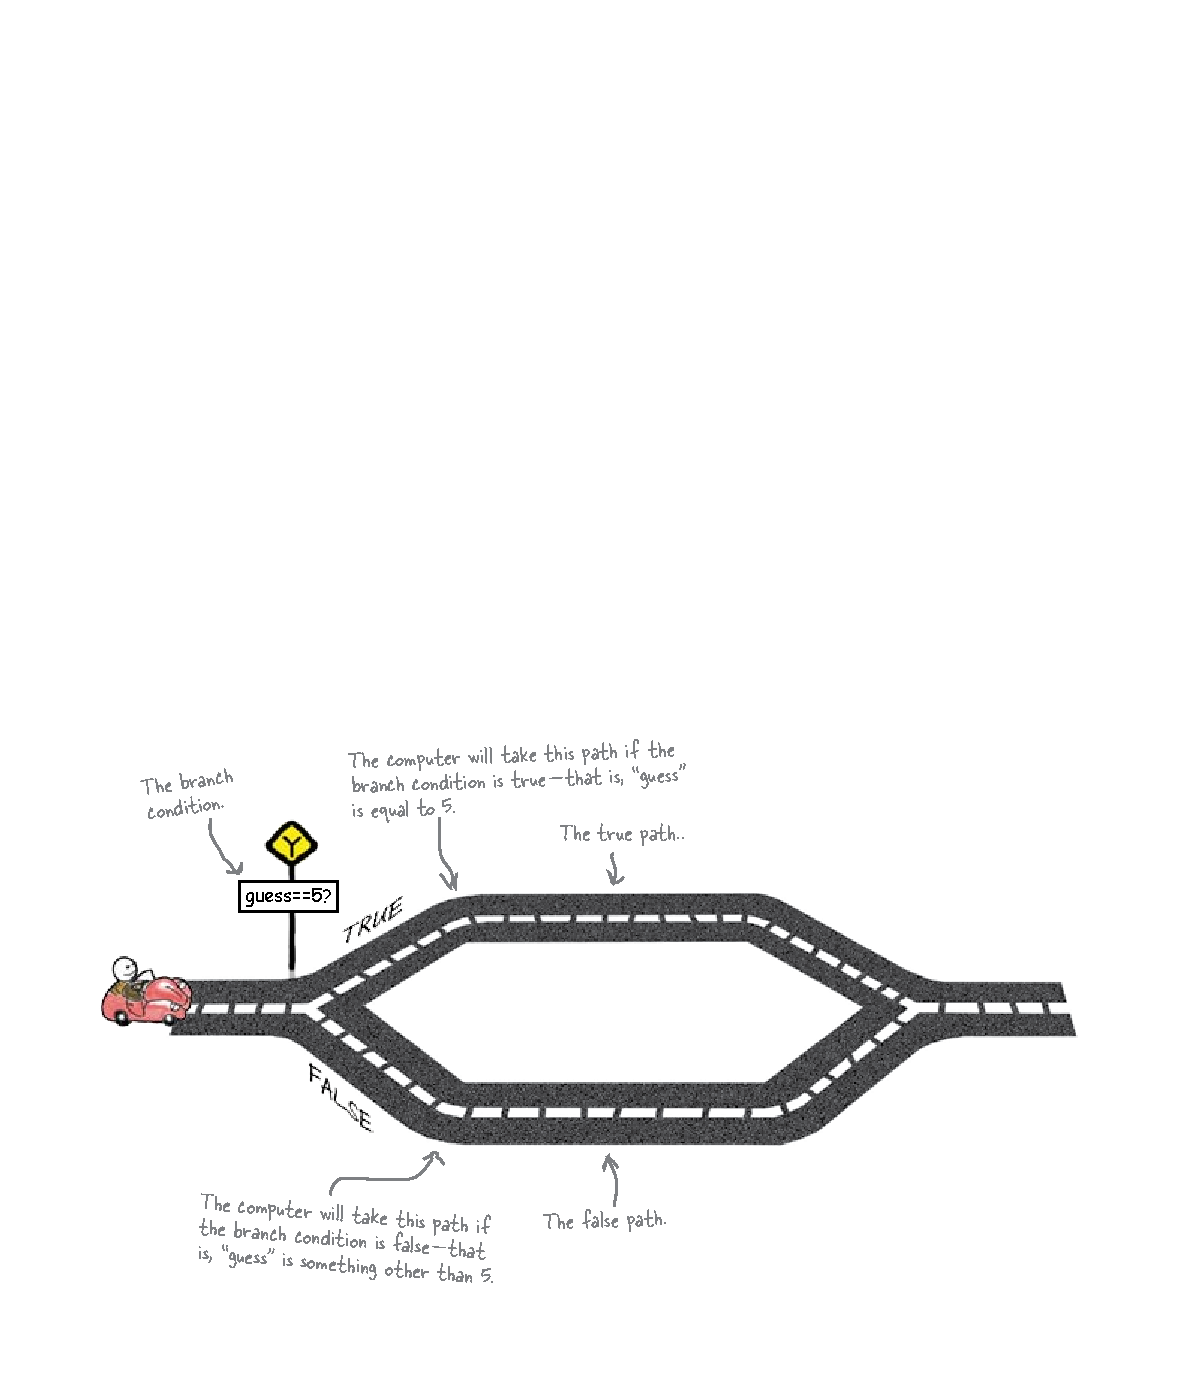
\includegraphics[width=0.8 \textwidth]{Branching}}
\end{itemize}
\end{frame}

\begin{frame}[fragile]
\frametitle{ \texttt{if} Statements}

 \texttt{if} statements have the following structure:
\begin{itemize}
\item The first line is the \alert{header}; the rest is the \alert{body}. 
\item The header has to end with a \alert{colon} and the body has to be \alert{indented}.
\item  By convention, the indentation is always \alert{four spaces}.  
\item The body can contain any number of statements.
\item Statements like this are called \alert{compound statements}.
%
%There is no limit on the number of statements that can appear in
%the body, but there has to be at least one.
%Occasionally, it is useful to have a body with no statements (usually
%as a place keeper for code you haven't written yet).  In that
%case, you can use the {\tt pass} statement, which does nothing.
%
\end{itemize}
\begin{block}{Example:Conditional Execution}
\tiny
\begin{verbatim}
if <test1> :
      <statements1>
\end{verbatim}
The \verb!<statements1>! are executed if \verb!<test1>! is \alert{true}.
\end{block}

\end{frame}

\begin{frame}[fragile]
\frametitle{Alternative Execution}
\begin{itemize}
\item Two possibilities and
the condition determines which one gets executed.
\item The alternatives are called
\alert{branches}, because they are branches in the flow of execution.
\end{itemize} 
 \begin{block}{Alternative Execution} 

\tiny
\begin{verbatim}
if <test1> :
    <statements1>
else:
    <statements2>
\end{verbatim}
\small
if \verb!<test1>! is \alert{true}, \verb!<statements1>! are executed; otherwise, 
\verb!<statements2>! are executed.
\end{block}

\end{frame}

\begin{frame}[fragile]
\frametitle{Multiway Branching}
\begin{itemize}
\item Sometimes there are more than two possibilities and we need more than
two branches.  
\item	Exactly one branch will be executed.  There is no limit on the number of \texttt{elif} statements. 
\item If there is an \texttt{else} clause, it has to be
at the \alert{end}.
\end{itemize}

\begin{block}{Example: Chained Conditionals} 
\tiny
\begin{verbatim}
if x < y:
    print 'x is less than y'
elif x > y:
    print 'x is greater than y'
else:
    print 'x and y are equal'
\end{verbatim}
\end{block}
\end{frame}



\begin{frame}[fragile]
\frametitle{Nested Conditionals}
\begin{itemize}
\item One conditional can also be \alert{nested} within another. 
\item In following example, the outer conditional contains two branches.  
\begin{itemize}[<+->]
\item The
first branch contains a simple statement.  
\item The second branch
contains another {\tt if} statement, which has \alert{two branches} of its
own.  
\item Those two branches are both simple statements,
although they could have been conditional statements as well.
\end{itemize}
\end{itemize}

\begin{block}{Example:Nested Conditionals} 
\tiny
\begin{verbatim}
if x == y:
    print 'x and y are equal'
else:
    if x < y:
        print 'x is less than y'
    else:
        print 'x is greater than y'
\end{verbatim}
\end{block}

\end{frame}

\begin{frame}[fragile]
\frametitle{Nested Conditionals}
\begin{itemize}
\item \alert{Logical operators} can be used to  simplify nested conditional
statements.  
\begin{block}{Nested \texttt{if}}
\tiny
\begin{verbatim}
if 0 < x:
    if x < 10:
        print 'x is a positive single-digit number.'
\end{verbatim}
\end{block}
%
\item The {\tt print} statement is executed only if we make it past \alert{ both}
conditionals, so we can get the same effect with the {\tt and} operator:

\begin{block}{Single Conditional}
\tiny
\begin{verbatim}
if 0 < x and x < 10:
    print 'x is a positive single-digit number.'
\end{verbatim}
\end{block}
\end{itemize}

\end{frame}


\begin{frame}[fragile]
\frametitle{\texttt{if} Statement: Example}
\begin{block}{Example}
\small
\begin{verbatim}
x=int(raw_input("Please enter an integer: ")) 
if x < 0 :
    x = 0
    print 'Negative changed to zero' 
elif x == 0:
    print 'Zero' 
elif x == 1:
    print 'Single' 
else:
    print 'More'
\end{verbatim}
\end{block}
%\begin{block}{}
%\begin{verbatim}
%>>>Please enter an integer: 42
%More
%>>>
%\end{verbatim}
%\end{block}
\end{frame}

\begin{frame}[fragile]
\frametitle{Indentation and Block Grouping}
\begin{itemize}
\item Leading whitespace (spaces and tabs) at the beginning of a line is used to compute the \alert{indentation level} of the line, which in turn is used to determine the \alert{grouping of statements}.
\item The total number of spaces preceding the first non-blank character then determines the line's indentation. 
\end{itemize}

\begin{block}{Example}
\tiny
\begin{verbatim}
def perm(l): # Compute the list of all permutations of l
    if len(l) <= 1: 
            return [l]
    r = [] 
    for i in range(len(l)):
         s = l[:i] + l[i+1:]
         p = perm(s) 
         for x in p:
          r.append(l[i:i+1] + x)
    return r
\end{verbatim}
\end{block}
\end{frame}
\section{Iteration}
\subsection{Simple Iteration}
\begin{frame}[fragile]
\frametitle{Iteration}
\begin{itemize} 
\item A common code pattern is \alert{iteration}, or \alert{looping}, which basically performs the same task in repetition.
\item In Python, two constructs are available for looping, \texttt{while} and \texttt{for}: 
\begin{itemize}
\item \texttt{while} : can be used to code \alert{general loops}.
\item \texttt{for}: is designed for stepping through the items in a \alert{ sequence object} and running a block of code for each. 
\end{itemize}
\end{itemize}
\begin{block}{General Loop Format}
\tiny
\begin{verbatim}
while <test1> :
    <statements1>
    if <test2>: break         #Exit loop now, skip else
    if <test3>: continue      #Go to top of loop now, to <test1>
else:
    <statements2>             # Run if we didn't hit a 'break'    
\end{verbatim}
\end{block}
\end{frame}
\begin{frame}[fragile]
\frametitle{\texttt{while} Statements}
\begin{itemize}
\item The flow of execution for a {\tt while} statement:

\begin{enumerate}
\item Initialize the  condition \alert{outside} the loop.
\item Evaluate the condition, yielding {\tt True} or {\tt False}.

\item If the condition is false, exit the {\tt while} statement
and continue execution at the next statement.

\item If the condition is true, execute the
body and then go back to step 2.
\end{enumerate}
\end{itemize}
\begin{block}{Example:Fibonacci Series}
\tiny
\begin{verbatim}
# Fibonacci series:
# the sum of two elements defines the next
a, b = 0, 1
while b < 10:
    print b
    a, b = b, a+b
\end{verbatim}
\end{block}
\end{frame}
\begin{frame}[fragile]
\frametitle{\texttt{break},\texttt{continue}}
\begin{itemize}
\item  Sometimes the loop needs to end half
way through the body.  Use the {\tt break}
statement to jump out of the \alert{closest enclosing} loop (past the entire loop statement).
\item Or you want to pass a block of the code and continue the iteration. Use the {\tt continue} statement to jump to the top of the \alert{closest enclosing} loop ( to the loop's header line).
\end{itemize}
\begin{block}{Example}
\tiny
\begin{verbatim}
while True:
    line = raw_input('> ')
    if line == 'done':
        break
    if line == 'no print': 
        continue
    print line
print 'Done!'
\end{verbatim}
\end{block}
\end{frame}
\begin{frame}[fragile]
\frametitle{loop \texttt{else}}
\begin{itemize}
\item Loop {\tt else} block runs  \alert{if and only if} the loop is exited normally (without hitting a \texttt{break}).
\end{itemize}
\begin{block}{Example}
\tiny
\begin{verbatim}
y=input('y= ')
x = y // 2
while x > 1:
    if y % x ==0:
        print( y, 'has factor', x)
        break
    x -=1
else:
    print(y, ' is prime')
\end{verbatim}
\end{block}
\end{frame}
\begin{frame}[fragile]
\frametitle{\texttt{for} Statements}
\begin{itemize}
\item The \texttt{for} statement iterates over the items of any sequence (a list or a string), in the order that they appear in the sequence.
\end{itemize}
\begin{block}{\texttt{for} example}
\begin{verbatim}
a = ['cat', 'window', 'defenestrate']
for x in a:
    print x, len(x)
\end{verbatim}
\end{block}
\end{frame}

\begin{frame}[fragile]
\frametitle{The \texttt{range()} function}
\begin{itemize}
\item Built-in function \texttt{range()} generates
lists containing arithmetic progressions.
\item The given end point is \alert{never} part of the generated list.
\begin{verbatim}
>>> range(10)
[0, 1, 2, 3, 4, 5, 6, 7, 8, 9]
>>> range(5, 10)
[5, 6, 7, 8, 9]
>>> range(0, 10, 3)
[0, 3, 6, 9]
>>> range(-10, -100, -30)
[-10, -40, -70]
\end{verbatim}
\end{itemize}

\end{frame}
\begin{frame}[fragile]
\frametitle{Looping using \texttt{for} and \texttt{range()}}
\begin{block}{Example}
\begin{verbatim}
for i in range(4):
     print 'Hello!'
\end{verbatim}
Output:
\begin{verbatim}
Hello!
Hello!
Hello!
Hello!
\end{verbatim}
\end{block}
\end{frame}

\end{document}


